% Options for packages loaded elsewhere
\PassOptionsToPackage{unicode}{hyperref}
\PassOptionsToPackage{hyphens}{url}
\documentclass[
]{article}
\usepackage{xcolor}
\usepackage{amsmath,amssymb}
\setcounter{secnumdepth}{-\maxdimen} % remove section numbering
\usepackage{iftex}
\ifPDFTeX
  \usepackage[T1]{fontenc}
  \usepackage[utf8]{inputenc}
  \usepackage{textcomp} % provide euro and other symbols
\else % if luatex or xetex
  \usepackage{unicode-math} % this also loads fontspec
  \defaultfontfeatures{Scale=MatchLowercase}
  \defaultfontfeatures[\rmfamily]{Ligatures=TeX,Scale=1}
\fi
\usepackage{lmodern}
\ifPDFTeX\else
  % xetex/luatex font selection
\fi
% Use upquote if available, for straight quotes in verbatim environments
\IfFileExists{upquote.sty}{\usepackage{upquote}}{}
\IfFileExists{microtype.sty}{% use microtype if available
  \usepackage[]{microtype}
  \UseMicrotypeSet[protrusion]{basicmath} % disable protrusion for tt fonts
}{}
\makeatletter
\@ifundefined{KOMAClassName}{% if non-KOMA class
  \IfFileExists{parskip.sty}{%
    \usepackage{parskip}
  }{% else
    \setlength{\parindent}{0pt}
    \setlength{\parskip}{6pt plus 2pt minus 1pt}}
}{% if KOMA class
  \KOMAoptions{parskip=half}}
\makeatother
\usepackage{longtable,booktabs,array}
\newcounter{none} % for unnumbered tables
\usepackage{calc} % for calculating minipage widths
% Correct order of tables after \paragraph or \subparagraph
\usepackage{etoolbox}
\makeatletter
\patchcmd\longtable{\par}{\if@noskipsec\mbox{}\fi\par}{}{}
\makeatother
% Allow footnotes in longtable head/foot
\IfFileExists{footnotehyper.sty}{\usepackage{footnotehyper}}{\usepackage{footnote}}
\makesavenoteenv{longtable}
\usepackage{graphicx}
\makeatletter
\newsavebox\pandoc@box
\newcommand*\pandocbounded[1]{% scales image to fit in text height/width
  \sbox\pandoc@box{#1}%
  \Gscale@div\@tempa{\textheight}{\dimexpr\ht\pandoc@box+\dp\pandoc@box\relax}%
  \Gscale@div\@tempb{\linewidth}{\wd\pandoc@box}%
  \ifdim\@tempb\p@<\@tempa\p@\let\@tempa\@tempb\fi% select the smaller of both
  \ifdim\@tempa\p@<\p@\scalebox{\@tempa}{\usebox\pandoc@box}%
  \else\usebox{\pandoc@box}%
  \fi%
}
% Set default figure placement to htbp
\def\fps@figure{htbp}
\makeatother
\setlength{\emergencystretch}{3em} % prevent overfull lines
\providecommand{\tightlist}{%
  \setlength{\itemsep}{0pt}\setlength{\parskip}{0pt}}
\usepackage{bookmark}
\IfFileExists{xurl.sty}{\usepackage{xurl}}{} % add URL line breaks if available
\urlstyle{same}
% fallback for those not using the hyperref driver hyperxmp:
\makeatletter
\@ifundefined{xmpquote}{\newcommand{\xmpquote}[1]{#1}}{}
\makeatother
\hypersetup{
  hidelinks,
  pdfcreator={LaTeX via pandoc}}

\author{}
\date{}

\begin{document}

\section{Day 23 Report --- PortSwigger Authentication
Lab}\label{day-23-report-portswigger-authentication-lab}

\subsection{Trios Cyber Internship}\label{trios-cyber-internship}

\textbf{Assignment:} PortSwigger Authentication Lab\\
\textbf{Lab:} 2FA simple bypass\\
\textbf{Platform:} PortSwigger Web Security Academy\\
\textbf{Tool:} Burp Suite\\
\textbf{Environment:} Kali Linux\\
\textbf{Status:} Completed\\
\textbf{Result:} Lab Solved

\begin{center}\rule{0.5\linewidth}{0.5pt}\end{center}

\subsection{1. Assignment Overview}\label{assignment-overview}

The Day 23 assignment required completing a beginner-level
authentication security lab and documenting relevant login and session
requests using Burp Suite.

The selected PortSwigger Web Security Academy lab was \textbf{2FA simple
bypass}, an intentionally vulnerable authentication training environment
designed to demonstrate improper enforcement of multi-factor
authentication.

\begin{center}\rule{0.5\linewidth}{0.5pt}\end{center}

\subsection{2. Objective}\label{objective}

The objectives of this exercise were:

\begin{enumerate}
\def\labelenumi{\arabic{enumi}.}
\tightlist
\item
  Understand the normal username/password authentication flow.
\item
  Observe the transition to the two-factor authentication stage.
\item
  Capture relevant authentication requests using Burp Suite.
\item
  Test whether access to the protected account page required completion
  of the second authentication factor.
\item
  Document the observed authentication weakness and its security
  implications.
\end{enumerate}

\begin{center}\rule{0.5\linewidth}{0.5pt}\end{center}

\subsection{3. Lab Environment}\label{lab-environment}

{\def\LTcaptype{none} % do not increment counter
\begin{longtable}[]{@{}ll@{}}
\toprule\noalign{}
Item & Details \\
\midrule\noalign{}
\endhead
\bottomrule\noalign{}
\endlastfoot
Operating System & Kali Linux \\
Web Security Tool & Burp Suite \\
Browser & Burp Suite built-in browser \\
Training Platform & PortSwigger Web Security Academy \\
Lab & 2FA simple bypass \\
Authentication Category & Multi-Factor Authentication \\
Target & Authorized PortSwigger training lab \\
\end{longtable}
}

All testing was conducted exclusively against the intentionally
vulnerable PortSwigger Web Security Academy environment.

\begin{center}\rule{0.5\linewidth}{0.5pt}\end{center}

\subsection{4. Lab Description}\label{lab-description}

The lab demonstrates a weakness in the enforcement of a two-factor
authentication process.

The application first accepts valid username/password credentials and
then redirects the user to a second-factor verification page.

The security test was to determine whether the authenticated session
could access the account page directly without completing the required
2FA step.

\begin{center}\rule{0.5\linewidth}{0.5pt}\end{center}

\subsection{5. Authentication Flow
Analysis}\label{authentication-flow-analysis}

The normal authentication flow observed through Burp Suite was:

\begin{verbatim}
POST /login
      |
      v
302 Found
      |
      v
GET /login2
      |
      v
4-digit 2FA code requested
\end{verbatim}

The initial login request used the lab-provided Wiener credentials:

\begin{verbatim}
username=wiener&password=peter
\end{verbatim}

The server responded with a redirect to:

\begin{verbatim}
/login2
\end{verbatim}

The /login2 page displayed a form requesting a 4-digit security code.

This established that the application expected a second authentication
factor after the initial username/password authentication.

\begin{center}\rule{0.5\linewidth}{0.5pt}\end{center}

\subsection{6. Burp Suite Request
Evidence}\label{burp-suite-request-evidence}

\subsubsection{6.1 Initial Login Request}\label{initial-login-request}

The initial authentication request was captured in Burp Suite HTTP
history:

\begin{verbatim}
POST /login HTTP/2
Host: <authorized PortSwigger lab host>

username=wiener&password=peter
\end{verbatim}

The server returned:

\begin{verbatim}
HTTP/2 302 Found
Location: /login2
\end{verbatim}

This demonstrated the transition from primary authentication to the
second-factor stage.

\subsubsection{6.2 Two-Factor Authentication
Stage}\label{two-factor-authentication-stage}

The following request was observed:

\begin{verbatim}
GET /login2 HTTP/2
Host: <authorized PortSwigger lab host>
\end{verbatim}

The response displayed a 4-digit MFA code input using the mfa-code
parameter.

This confirmed that the application had moved the user into the 2FA
stage.

\begin{center}\rule{0.5\linewidth}{0.5pt}\end{center}

\subsection{7. Carlos Account
Authentication}\label{carlos-account-authentication}

The lab supplied a separate training account for the victim user:

\begin{verbatim}
Username: carlos
Password: montoya
\end{verbatim}

After authenticating with these credentials, the application again
presented the /login2 2FA verification page.

At this point, the second authentication factor had not been completed.

No attempt was made to obtain, guess, or bypass the security code
itself.

\begin{center}\rule{0.5\linewidth}{0.5pt}\end{center}

\subsection{8. Direct Account-Page Access
Test}\label{direct-account-page-access-test}

The key security test was performed by requesting the account page
directly without submitting a 2FA code:

\begin{verbatim}
GET /my-account
\end{verbatim}

Instead of requiring completion of the /login2 stage, the application
allowed access to the authenticated account page.

The PortSwigger Web Security Academy subsequently displayed the lab as
Solved.

This confirmed that the second authentication factor was not being
adequately enforced before access to the protected account resource.

\begin{center}\rule{0.5\linewidth}{0.5pt}\end{center}

\subsection{9. Vulnerability Analysis}\label{vulnerability-analysis}

The observed behavior represents a \textbf{2FA bypass caused by
insufficient server-side enforcement of the second authentication
factor}.

The application correctly displayed a 2FA step during the normal login
flow, but access control for the protected account page did not
sufficiently verify that the second authentication factor had been
completed.

In practical terms, successful completion of the first authentication
step was sufficient to reach a protected resource that should have
required completion of the second factor.

\begin{center}\rule{0.5\linewidth}{0.5pt}\end{center}

\subsection{10. Security Impact}\label{security-impact}

If a similar weakness existed in a real-world application, an attacker
who obtained valid primary authentication credentials could potentially
access resources intended to be protected by multi-factor
authentication.

This could reduce the security benefit provided by 2FA and potentially
expose authenticated account functionality.

The actual impact in a production application would depend on the
resources protected by the affected authentication mechanism.

\begin{center}\rule{0.5\linewidth}{0.5pt}\end{center}

\subsection{11. Recommended Mitigation}\label{recommended-mitigation}

Applications implementing multi-factor authentication should enforce the
second authentication factor on the server side before granting access
to protected resources.

Recommended controls include:

\begin{itemize}
\tightlist
\item
  Maintain a server-side authentication state indicating whether MFA has
  been successfully completed.
\item
  Require the MFA-completed state before serving protected account
  pages.
\item
  Do not rely solely on client-side redirects or the visible /login2
  page.
\item
  Validate authorization requirements on every protected endpoint.
\item
  Invalidate or restrict partially authenticated sessions appropriately.
\item
  Test direct access to protected endpoints during authentication
  security assessments.
\end{itemize}

\begin{center}\rule{0.5\linewidth}{0.5pt}\end{center}

\subsection{12. Evidence Collected}\label{evidence-collected}

{\def\LTcaptype{none} % do not increment counter
\begin{longtable}[]{@{}
  >{\raggedright\arraybackslash}p{(\linewidth - 2\tabcolsep) * \real{0.5000}}
  >{\raggedright\arraybackslash}p{(\linewidth - 2\tabcolsep) * \real{0.5000}}@{}}
\toprule\noalign{}
\begin{minipage}[b]{\linewidth}\raggedright
Evidence
\end{minipage} & \begin{minipage}[b]{\linewidth}\raggedright
Purpose
\end{minipage} \\
\midrule\noalign{}
\endhead
\bottomrule\noalign{}
\endlastfoot
01-authentication-lab-open.png & Documents the selected authentication
lab \\
02-login-request-burp.png & Shows the primary login request in Burp \\
03-login2-mfa-stage.png & Shows the 2FA verification stage \\
04-authentication-bypass.png & Shows successful direct account access
and solved lab \\
\end{longtable}
}

Raw request-flow documentation was preserved in:

\begin{verbatim}
logs/authentication-session-flow.txt
\end{verbatim}

\begin{center}\rule{0.5\linewidth}{0.5pt}\end{center}

\subsection{13. Evidence Screenshots}\label{evidence-screenshots}

\subsubsection{13.1 Authentication Lab}\label{authentication-lab}

\begin{figure}
\centering
\pandocbounded{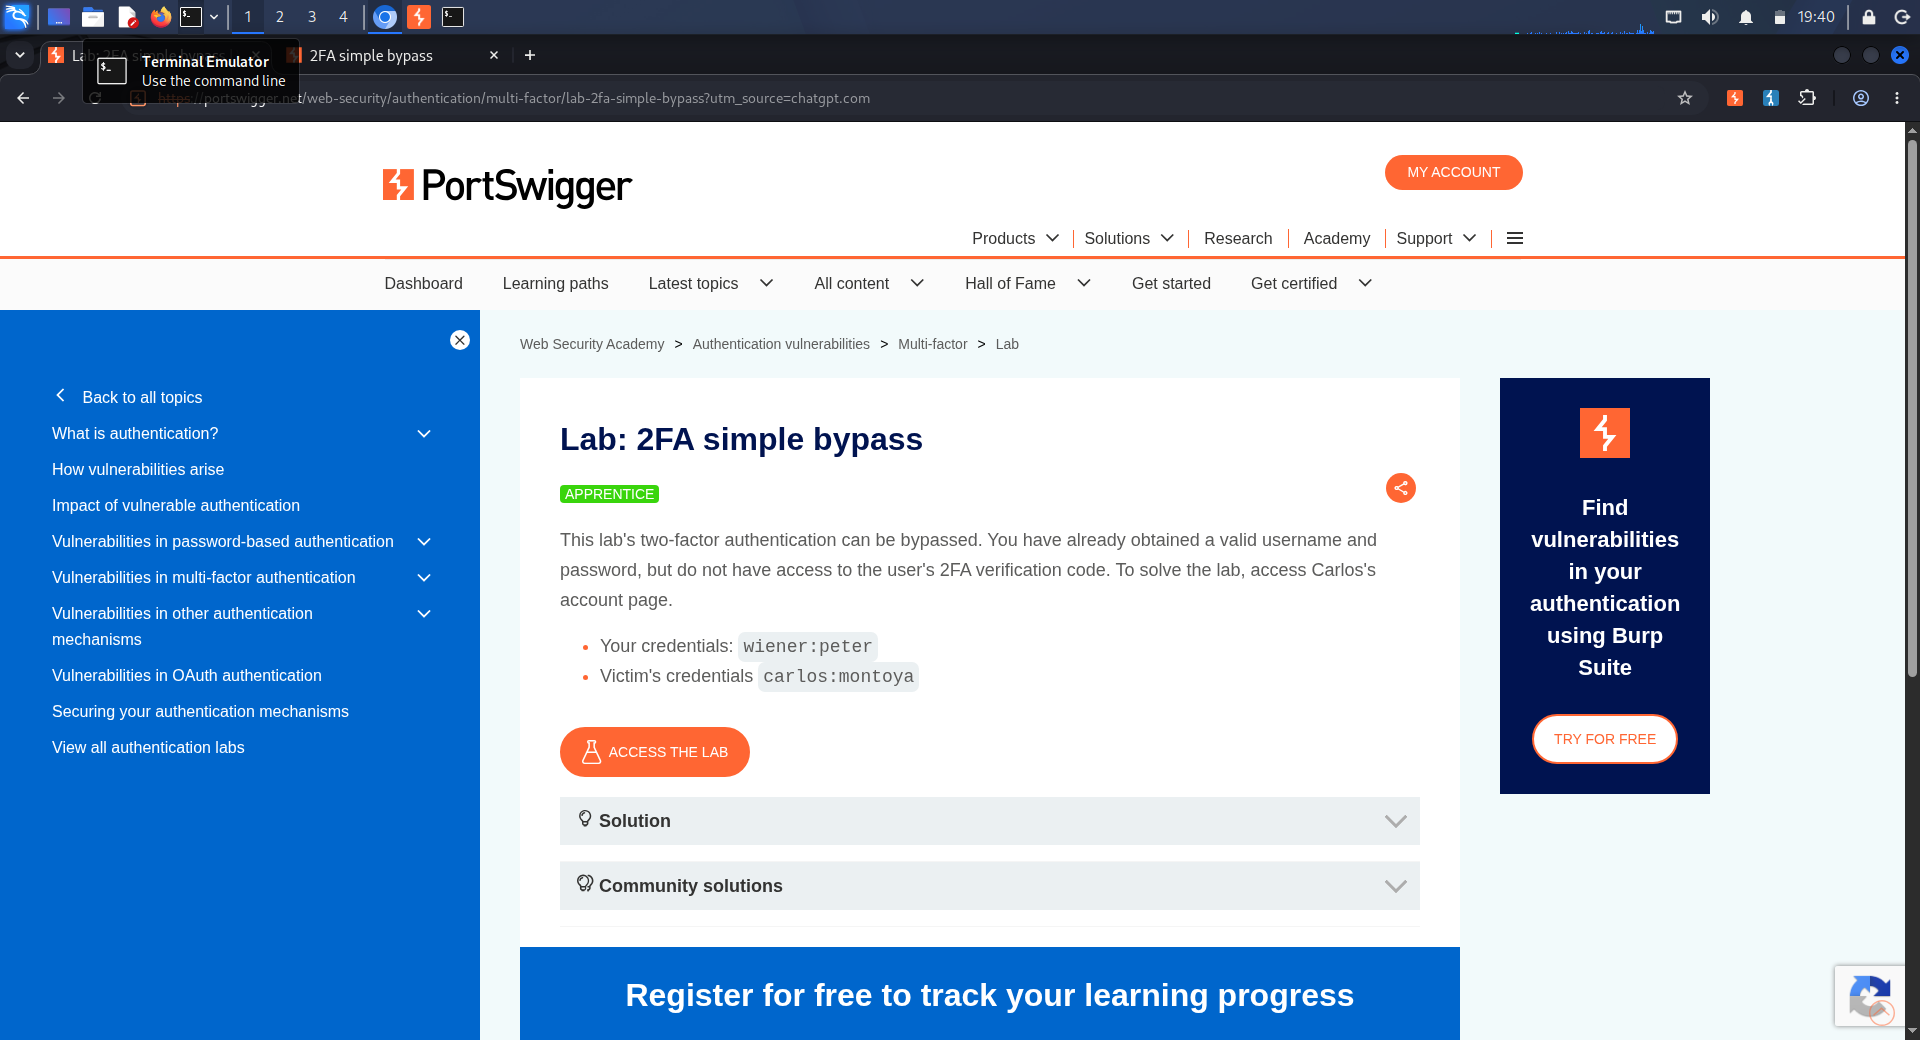
\includegraphics[keepaspectratio,alt={PortSwigger authentication lab}]{screenshots/01-authentication-lab-open.png}}
\caption{PortSwigger authentication lab}
\end{figure}

\subsubsection{13.2 Login Request in Burp
Suite}\label{login-request-in-burp-suite}

\begin{figure}
\centering
\pandocbounded{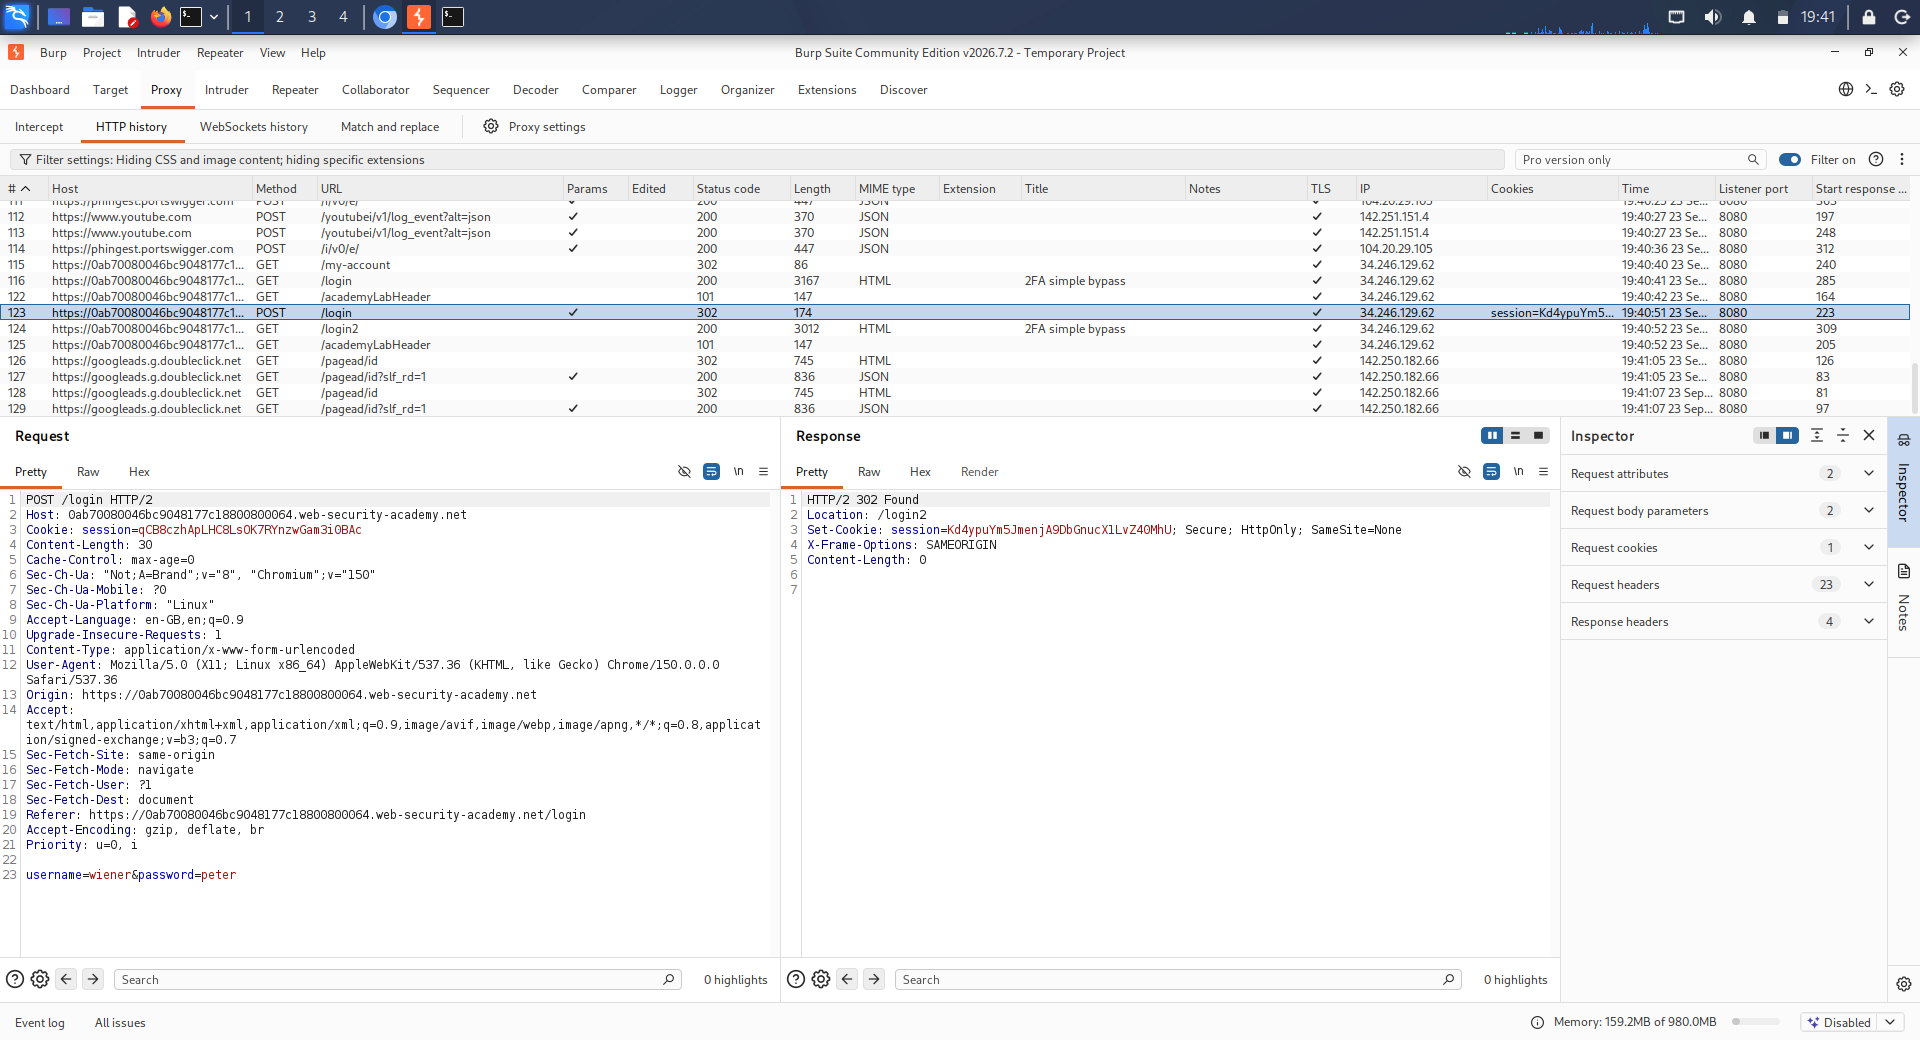
\includegraphics[keepaspectratio,alt={Primary login request captured in Burp Suite}]{screenshots/02-login-request-burp.png}}
\caption{Primary login request captured in Burp Suite}
\end{figure}

\subsubsection{13.3 Two-Factor Authentication
Stage}\label{two-factor-authentication-stage-1}

\begin{figure}
\centering
\pandocbounded{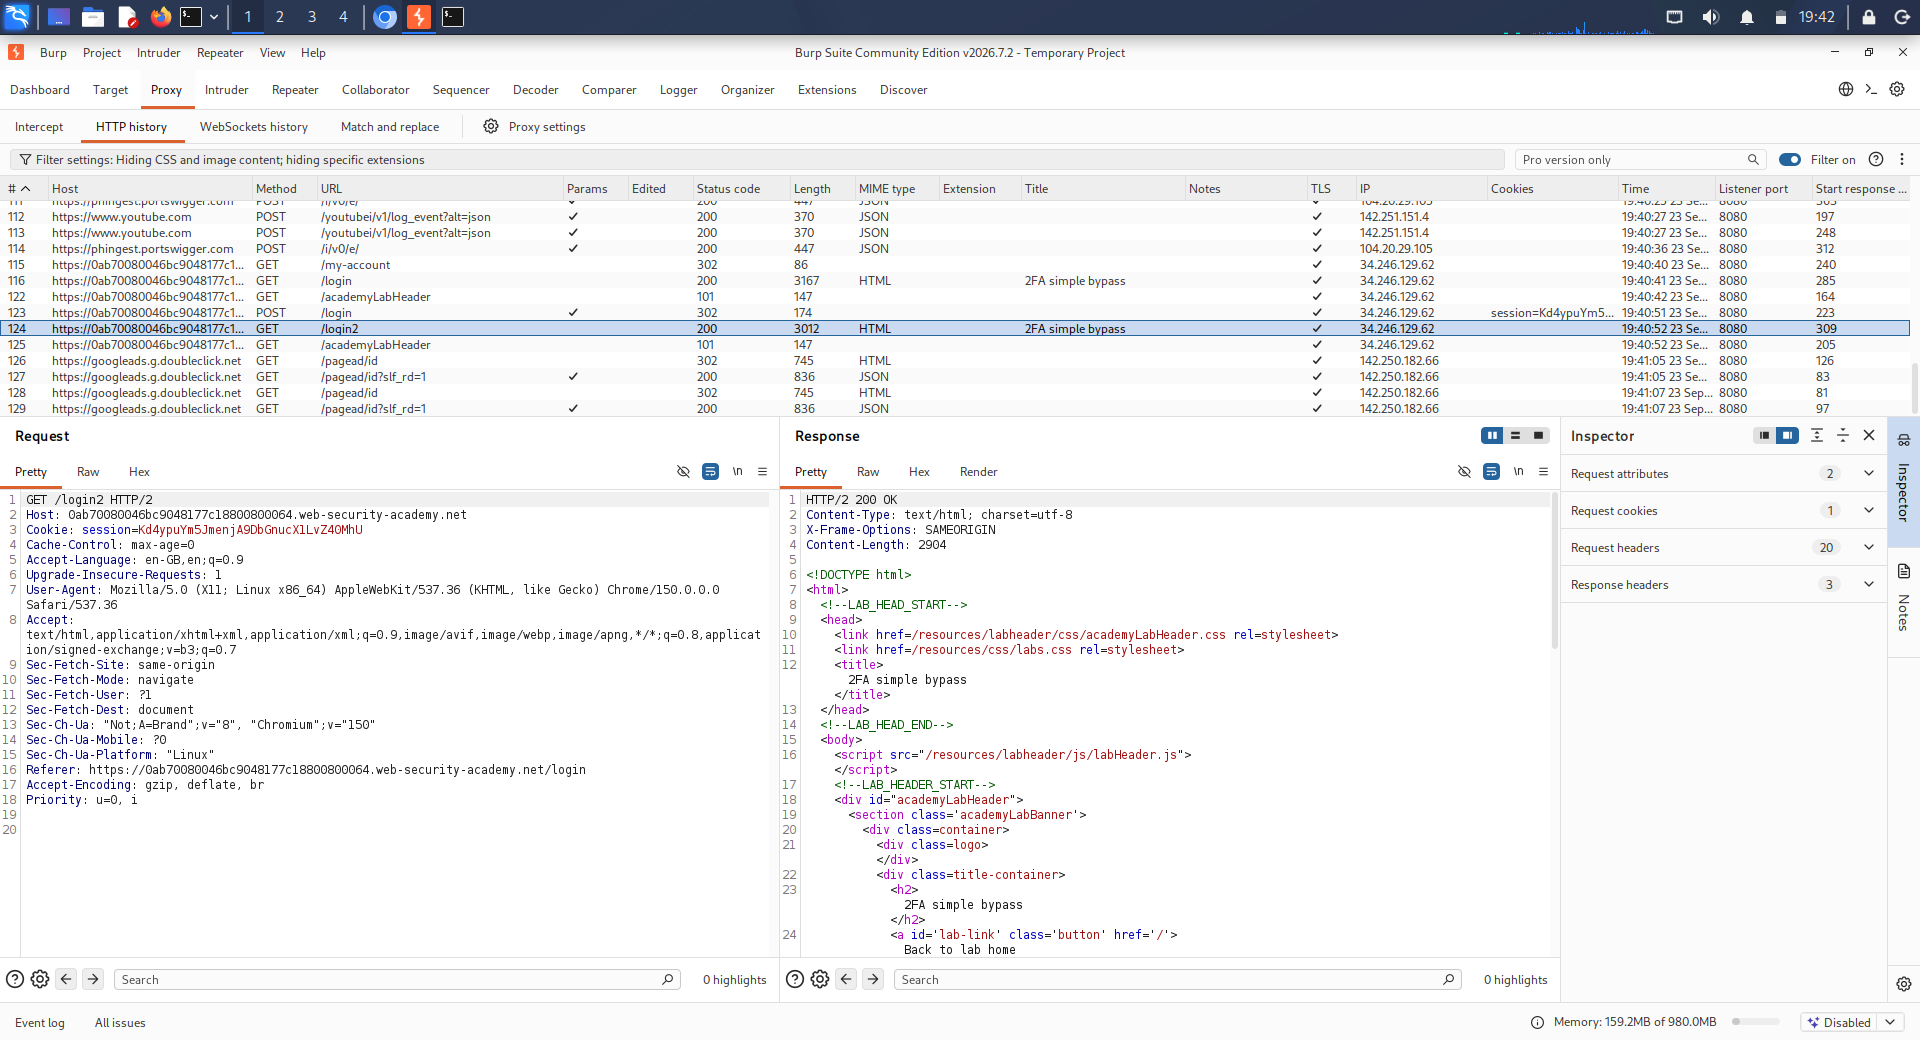
\includegraphics[keepaspectratio,alt={2FA verification stage}]{screenshots/03-login2-mfa-stage.png}}
\caption{2FA verification stage}
\end{figure}

\subsubsection{13.4 Successful Authentication
Bypass}\label{successful-authentication-bypass}

\begin{figure}
\centering
\pandocbounded{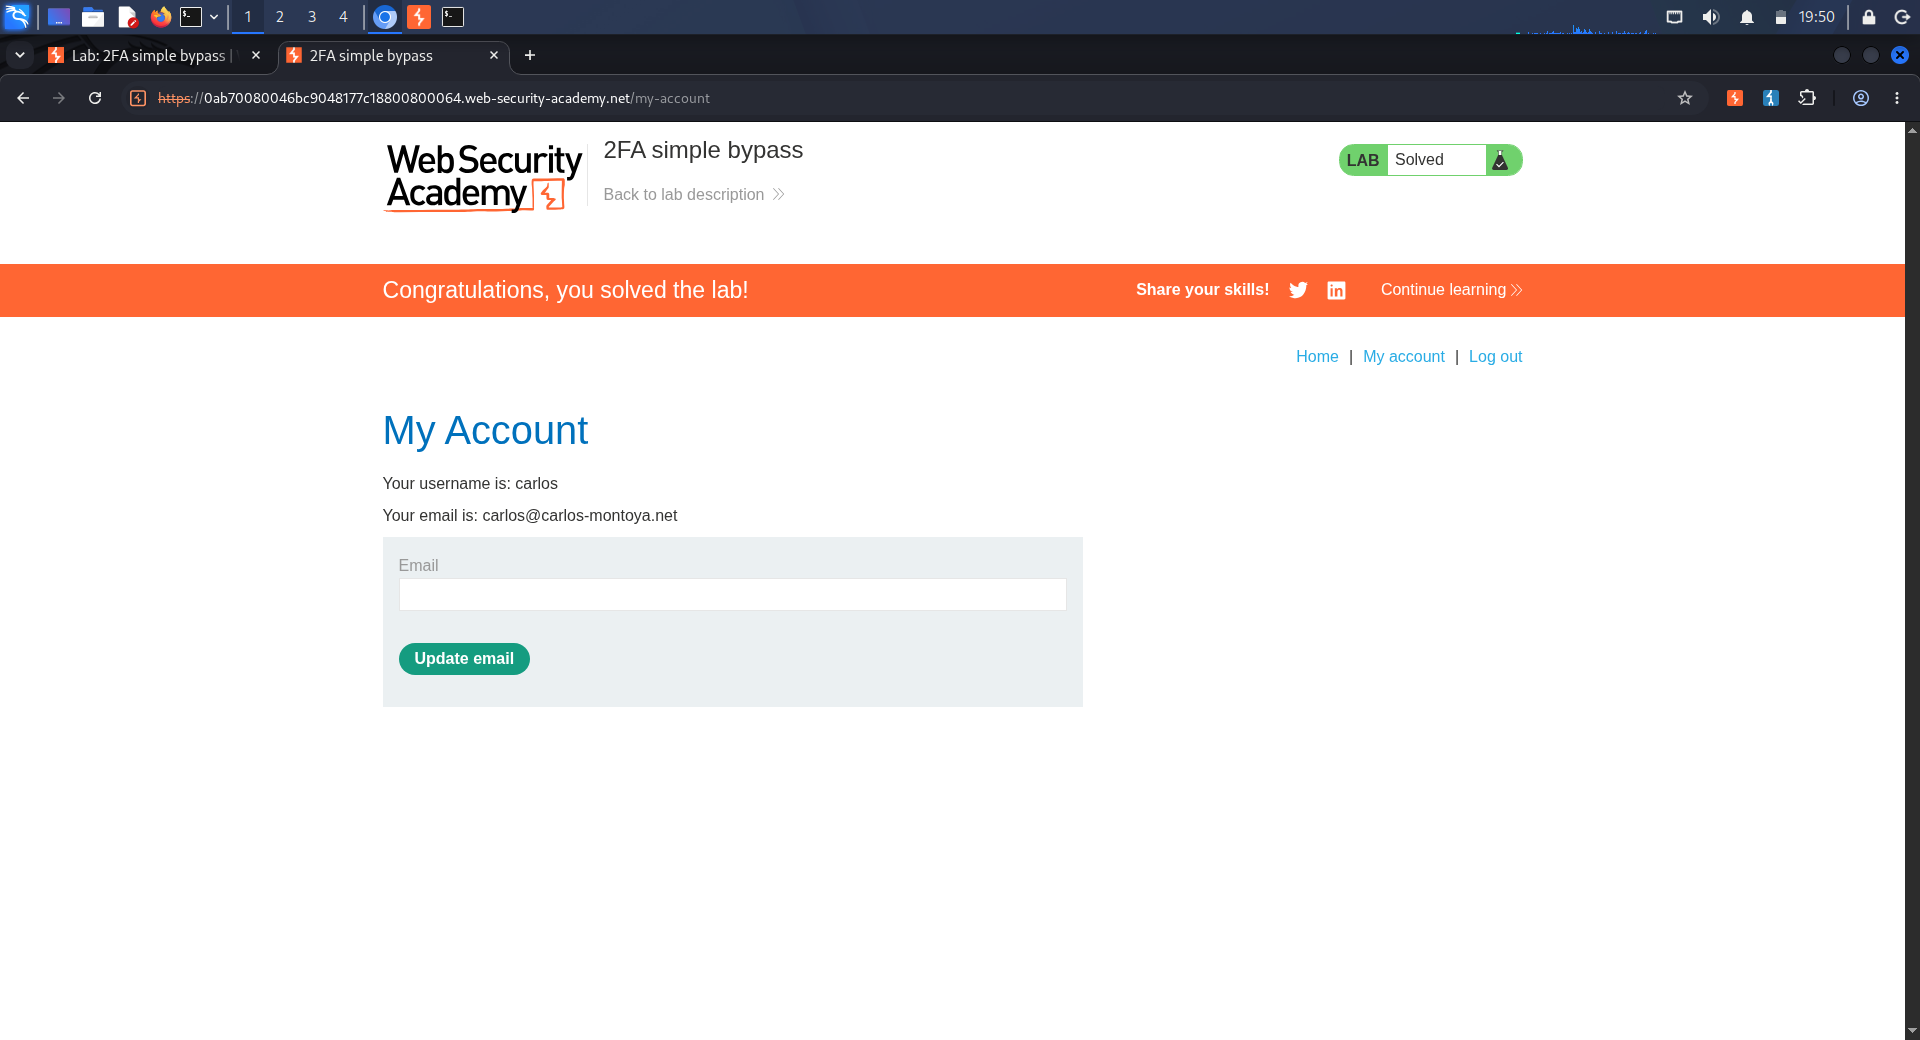
\includegraphics[keepaspectratio,alt={Successful direct account access and solved lab}]{screenshots/04-authentication-bypass.png}}
\caption{Successful direct account access and solved lab}
\end{figure}

\begin{center}\rule{0.5\linewidth}{0.5pt}\end{center}

\subsection{14. Key Learning Outcomes}\label{key-learning-outcomes}

This exercise demonstrated:

\begin{enumerate}
\def\labelenumi{\arabic{enumi}.}
\tightlist
\item
  How username/password authentication can transition into an MFA stage.
\item
  How Burp Suite HTTP history can be used to inspect authentication
  requests.
\item
  The difference between displaying an MFA challenge and actually
  enforcing MFA.
\item
  Why protected endpoints must independently validate authentication
  state.
\item
  How direct endpoint testing can reveal authentication enforcement
  weaknesses.
\item
  The importance of documenting both normal authentication behavior and
  security-test results.
\end{enumerate}

\begin{center}\rule{0.5\linewidth}{0.5pt}\end{center}

\subsection{15. Conclusion}\label{conclusion}

The PortSwigger \textbf{2FA simple bypass} lab was successfully
completed using Burp Suite.

The assessment identified that the application allowed direct access to
the protected account page without completing the required 2FA step. The
PortSwigger Academy confirmed the result by marking the lab as Solved.

The exercise provided practical experience in analyzing authentication
flows, inspecting HTTP requests, and identifying weaknesses in
server-side multi-factor authentication enforcement.

\begin{center}\rule{0.5\linewidth}{0.5pt}\end{center}

\subsection{16. Scope and Authorization}\label{scope-and-authorization}

All testing described in this report was performed exclusively against
the intentionally vulnerable PortSwigger Web Security Academy training
environment.

No unauthorized systems, services, or real-world accounts were targeted.

\end{document}
